\chapter{Preliminary exploration of underwater IPT system}

% 为了探究实际情况中海水环境下的无线能量传输系统与空气中的无线能量传输系统的异同,这里使用了简单的双线圈结构对水下环境的电气属性进行了探究。本章将介绍双线圈结构在海水中工作的表现。
In order to explore the similarities and differences between the wireless energy transmission system in the seawater environment and the wireless energy transmission system in the air in the actual situation, a simple double-coil structure is used to explore the electrical properties of the underwater environment. This chapter will introduce the performance of the double coil structure working in sea water.




\section{The system in three different media}

\begin{figure}[!b]
    \resizebox*{\textwidth}{!}{
    \begin{subfigure}{0.5\textwidth}
        \centering
        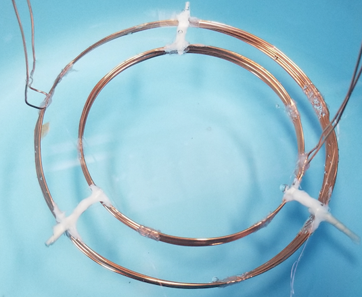
\includegraphics[width=0.9\linewidth, height=5.4cm]{images/3_two_ring_coil.png}
        \caption{Experimental coil.}
        \label{fig:subim1}
    \end{subfigure}
    \begin{subfigure}{0.5\textwidth}
        \centering
        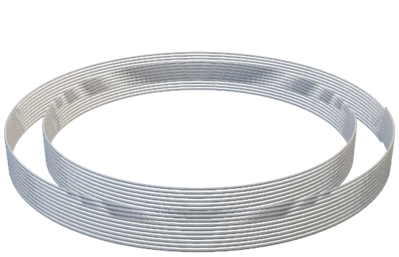
\includegraphics[width=0.9\linewidth, height=5.4cm]{images/3_two_ring_coil_structure.png}
        \caption{Structure diagram.}
        \label{fig:subim2}
    \end{subfigure}
    }
    \caption{Two ring structure.}
    \label{fig:3_two_ring_coil}
\end{figure}

In order to design a wireless power transmission system suitable for underwater AUV, we will first use hollow cylindrical structure transmitter and cylindrical structure receiver to explore the performance of the UWPT system of this plug-in structure UWPT in water. For the convenience of writing, it will be referred to as a double ring structure in the following text. The coil structure as shown in figure \ref{fig:3_two_ring_coil}.

Its detailed parameters are shown in Table \ref{table:ring coil parameters}.

\begin{table}[!t]
    \centering
    \caption{The parameters of ring coil structure.}
    \begin{tabular}{ c|cc }
        \thickhline
        % \hline
        \textbf{Items}                    & \textbf{Parameters}      \\
        \thickhline
        Environment                       & Air, tap water, seawater \\ \hline
        Wire diameter                     & 0.8mm                    \\ \hline
        Wire material                     & Copper                   \\
        \hline
        Tx coil diameter                  & 113mm                    \\ \hline
        Rx coil diameter                  & 85mm                     \\ \hline
        Turns (Inner coil and outer coil) & 10                       \\ \hline
        Frequency                         & 200kHz                   \\ \hline
    \end{tabular}
    \label{table:ring coil parameters}
\end{table}

% 当我们使用VNA分析仪将线圈放置在空气中,自来水中,海水中进行测量时,可以得到以下数据
When we use the VNA analyzer to place the coil in the air, tap water, or sea water for measurement, the following data can be obtained:
\begin{equation*}
    \begin{aligned}
        Z_{air}       & =
        \begin{bmatrix}
            0.4 +29.6i & 0.0 -10.0i \\
            0.0 -10.0i & 0.3 +20.3i
        \end{bmatrix}, \\
        Z_{tap-water} & =
        \begin{bmatrix}
            3.0 +32.1i  & -1.5 -11.3i \\
            -1.5 -11.3i & 1.5 +21.6i
        \end{bmatrix}, \\
        Z_{seawater}  & =
        \begin{bmatrix}
            7.2 +37.8i  & -6.0 -15.7i \\
            -6.0 -15.7i & 6.5 +25.3i
        \end{bmatrix}.
    \end{aligned}
\end{equation*}

In the above measurement results, we can find that as the transmission medium changes (from air to tap-water to seawater), each corresponding value is increasing.
It illustrates that the internal resistances of the coils are small in the air.
However, the internal resistances significantly increase when the coils are in tapwater or seawater.
This may deteriorate the transmission efficiency as well as the load voltage stability.
In addition, the mutual inductance between two coils becomes complex number and the self-inductances of the coils slightly increase. 

\section{The system in different sizes of the coil}

\begin{figure}[!t]
    \centering
    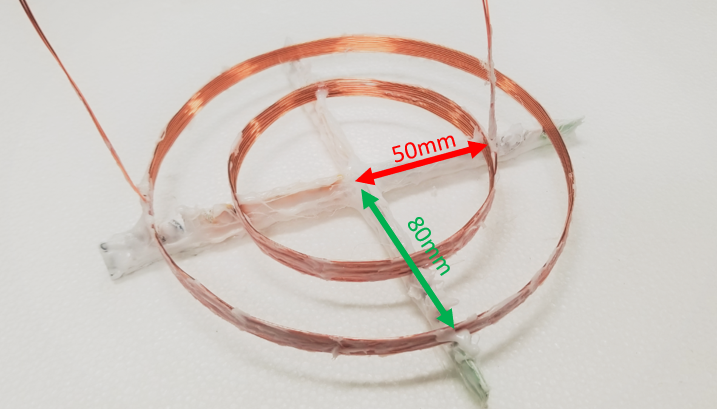
\includegraphics[width=0.9\linewidth]{images/3_two_ring_coil_5cm_8cm.png}
    \caption{Two ring structure ($r_{inner}=50mm$, $r_{outer}=80mm$).}
    \label{fig:3_two_ring_coil_5cm_8cm}
\end{figure}

In order to explore the influence of the size of the internal coil and the distance between the two coils on the system (Figure \ref{fig:3_two_ring_coil_5cm_8cm}), the coil size is changed here to change the distance between the transmitter and the receiver. The specific parameters are as follows (Table \ref{table:ring coil parameters - different distance}).

\begin{table}[!b]
    \centering
    \caption{The parameters of ring coil structure.}
    \begin{tabular}{ c|cc }
        \thickhline
        % \hline
        \textbf{Items}                    & \textbf{Parameters}      \\
        \thickhline
        Environment                       & Air, tap water, seawater \\ \hline
        Wire diameter                     & 0.8mm                    \\ \hline
        Wire material                     & Copper                   \\
        \hline
        Tx coil diameter                  & 160mm                    \\ \hline
        Rx coil diameter                  & 100mm, 120mm, 140mm      \\ \hline
        Turns (Inner coil and outer coil) & 10                       \\ \hline
        Frequency                         & 200kHz                   \\ \hline
    \end{tabular}
    \label{table:ring coil parameters - different distance}
\end{table}

After changing the medium between the coils and the distance between the coils, the Z-parameters in different scenarios are measured by VNA, and we get the following results (Table \ref{table:Z-parameters in distance}).

\newcommand\Tstrut{\rule{0pt}{2.3em}}         % = `top' strut
\newcommand\Bstrut{\rule[-1.8em]{0pt}{0pt}}   % = `bottom' strut

\begin{table}[!t]
    \centering
    \caption{Z-parameters in different distance and media}
    % \renewcommand{\arraystretch}{1}
    % \setlength\extrarowheight{10pt}
    \resizebox*{\textwidth}{!}{
    \begin{tabular}{|c|c|c|c|}
        \hline
        \textbf{Media}             & \textbf{\begin{tabular}[c]{@{}c@{}}Coil size\\ (Radius)\end{tabular}} & \textbf{Distance} & \textbf{Z-parameter}         \\ \hline
        \multirow{3}{*}{Air}       & 80mm - 50mm                        & 30mm              & $\begin{bmatrix} 0.6826 + 46.4075i & -0.0411-8.9620i \\ -0.0382-8.9669i            &0.3423+24.2260i  \end{bmatrix}$ \Tstrut\Bstrut\\ \cline{2-4}
                                   & 80mm - 60mm                        & 20mm              & $\begin{bmatrix} 0.7194	+46.1416i  & -0.0946	-15.0048i \\
                -0.0906	-15.0155i & 0.5225	+32.5246i\end{bmatrix}$ \Tstrut\Bstrut\\ \cline{2-4}
                                   & 80mm - 70mm                        & 10mm              & $\begin{bmatrix} 0.6657	+45.9561i & 0.0757	+24.2562i \\
                0.0699	+24.2747i & 0.5651	+39.2948i\end{bmatrix}$ \Tstrut\Bstrut\\ \hline
        \multirow{3}{*}{Tap-water} & 80mm - 50mm                        & 30mm              & $\begin{bmatrix} 5.4603	+53.0814i  & -2.4332	-11.7753i \\
                -2.4304	-11.7859i & 1.7722	+26.0449i\end{bmatrix}$ \Tstrut\Bstrut\\ \cline{2-4}
                                   & 80mm - 60mm                        & 20mm              & $\begin{bmatrix} 7.0513	+54.2993i  & -4.4889	-20.1926i \\
                -4.4867	-20.2100i & 3.9114	+36.7652i\end{bmatrix}$ \Tstrut\Bstrut\\ \cline{2-4}
                                   & 80mm - 70mm                        & 10mm              & $\begin{bmatrix} 2.8768	+49.8765i & 0.9991	+26.5644i \\
                0.9946	+26.5864i & 1.9865	+42.0751i\end{bmatrix}$ \Tstrut\Bstrut\\ \hline
        \multirow{3}{*}{Seawater}  & 80mm - 50mm                        & 30mm              & $\begin{bmatrix} 1.761	+58.2022i   & -0.554	-14.5303i \\
                -0.5512	-14.5424i & 0.6543	+27.6708i\end{bmatrix}$ \Tstrut\Bstrut\\ \cline{2-4}
                                   & 80mm - 60mm                        & 20mm              & $\begin{bmatrix} 2.0488	+61.1579i  & -0.9906	-25.1528i \\
                -0.9814	-25.1736i & 1.2212	+40.4982i\end{bmatrix}$ \Tstrut\Bstrut\\ \cline{2-4}
                                   & 80mm - 70mm                        & 10mm              & $\begin{bmatrix} 2.0347	+52.4298i & 0.4957	+27.1092i \\
                0.4843	+27.1321i & 1.4439	+43.4828i\end{bmatrix}$ \Tstrut\Bstrut\\ \hline
    \end{tabular}
    }
    \renewcommand{\arraystretch}{1}
    \label{table:Z-parameters in distance}
\end{table}

% 结论
% 在这个表格中,我们可以发现,在同种介质下,随着内部线圈减小,传输距离增加,我们可以看到Z11的虚部和Z22的虚部在增大,表明线圈的阻抗正在增大。

In table \ref{table:Z-parameters in distance}, we can find that under the same medium, as the internal coil decreases, the transmission distance increases. We can see that the imaginary part of $Z_{11}$ and $Z_{22}$ are increasing, indicating that the impedance of the coil is increasing.

Table \ref{table:Z-parameters in distance} shows the measures of Z-parameter of the coupling network under several cases of coil sizes and distances in air, tap-water and seawater.
In general, self-inductance of coil increases as coil size increases.
The mutual inductance between two coils increases as the distance between them decreases.
The internal resistances of the coils are small in air and larger in tapwater as well as seawater.

\section{The system in different frequency}
Earlier we have studied the z-parameter changes of the two ring coil structure under different media and different distances. In this section we will study how z-parameters changes at different frequencies. Table \ref{table:ring coil parameters - different frequencies} a shows the parameters of the experiment.

\begin{table}[!t]
    \centering
    \caption{The parameters of ring coil structure.}
    \begin{tabular}{ c|cc }
        \thickhline
        % \hline
        \textbf{Items}                    & \textbf{Parameters}                    \\
        \thickhline
        Environment                       & Air, seawater                          \\ \hline
        Wire diameter                     & 0.8mm                                  \\ \hline
        Wire material                     & Copper                                 \\
        \hline
        Tx coil diameter                  & 160mm                                  \\ \hline
        Rx coil diameter                  & 100mm                                  \\ \hline
        Turns (Inner coil and outer coil) & 10                                     \\ \hline
        Frequency                         & 100kHz, 150kHz, 200kHz, 250kHz, 300kHz \\ \hline
    \end{tabular}
    \label{table:ring coil parameters - different frequencies}
\end{table}

After using the above parameters, we got the following results (Table \ref{table:ring Z-parameters - different frequencies}).
% 结果表格

\begin{table}[!t]
    \centering
    \caption{Z-parameters in different frequencies and media}
    \begin{tabular}{|c|c|c|c|}
        \hline
        \textbf{Media}            & \textbf{Frequency} & \textbf{Z-parameter}                  \\ \hline
        \multirow{5}{*}{Air}      & 100kHz             & $\begin{bmatrix}
                0.3758 +23.2130i  & -0.0036 - 4.4495i \\
                -0.0012 - 4.4520i & 0.2123 +12.1526i
            \end{bmatrix}$          \Tstrut\Bstrut\\ \cline{2-3}
                                  & 150kHz             & $\begin{bmatrix}
                0.4789 +34.7320i  & -0.0074 - 6.6739i \\
                -0.0037 - 6.6774i & 0.2575 +18.1971i
            \end{bmatrix}$          \Tstrut\Bstrut\\ \cline{2-3}
                                  & 200kHz             & $\begin{bmatrix}
                0.5755 +46.2288i  & -0.0121 - 8.9004i \\
                -0.0050 - 8.9065i & 0.3031 +24.2211i
            \end{bmatrix}$          \Tstrut\Bstrut\\ \cline{2-3}
                                  & 250kHz             & $\begin{bmatrix}
                0.6737 +57.7432i  & -0.0153 -11.1342i \\
                -0.0095 -11.1426i & 0.3423 +30.2465i
            \end{bmatrix}$          \Tstrut\Bstrut\\ \cline{2-3}
                                  & 300kHz             & $\begin{bmatrix}
                0.7556 +69.2691i  & -0.0191 -13.3746i \\
                -0.0100 -13.3859i & 0.3791 +36.2676i
            \end{bmatrix}$          \Tstrut\Bstrut\\ \hline
        \multirow{5}{*}{Seawater} & 100kHz             & $\begin{bmatrix}
                0.5314 +24.3255i  & -0.0760 - 4.9832i \\
                -0.0717 - 4.9862i & 0.2593 +12.5247i
            \end{bmatrix}$          \Tstrut\Bstrut\\ \cline{2-3}
                                  & 150kHz             & $\begin{bmatrix}
                0.9900 +39.2700i  & -0.2453 - 8.8345i \\
                -0.2392 - 8.8400i & 0.4080 +19.6434i
            \end{bmatrix}$          \Tstrut\Bstrut\\ \cline{2-3}
                                  & 200kHz             & $\begin{bmatrix}
                2.0236 +59.0193i  & -0.7053 -15.0451i \\
                -0.6942 -15.0581i & 0.7248 +28.1895i
            \end{bmatrix}$          \Tstrut\Bstrut\\ \cline{2-3}
                                  & 250kHz             & $\begin{bmatrix}
                4.8486 +89.4034i  & -2.0763 -26.6084i \\
                -2.0597 -26.6276i & 1.5345 +39.8440i
            \end{bmatrix}$          \Tstrut\Bstrut\\ \cline{2-3}
                                  & 300kHz             & $10^2 \times \begin{bmatrix}
                0.1548 + 1.4909i  & -0.0751 - 0.5327i \\
                -0.0749 - 0.5333i & 0.0450 + 0.5985i
            \end{bmatrix}$ \Tstrut\Bstrut\\ \hline
    \end{tabular}
    \label{table:ring Z-parameters - different frequencies}
\end{table}

Table \ref{table:ring Z-parameters - different frequencies} shows that the internal resitances of the coils are less than $1\si{\ohm}$ in the air when operating frequency changes from $100\si{\kilo\hertz}$ to $300\si{\kilo\hertz}$.
However, under seawater environment, the internal resistances of the coils are smaller than $1\si{\ohm}$ when the operating frequency is under $200\si{\kilo\hertz}$.
As the operating frequency is over $200\si{\kilo\hertz}$, the internal resistances of the coils significantly increase.


\section{Conclusion}

This section illustrated the measures of the coupling network in air, under tapwater and under seawater with different operating frequencies.
The measures indicated that the internal resistances of the coils would increase when the system operated under tapwater or seawater.
This would reduce transmission efficiency.
Moreoever, it could also make load voltage unstable against load variations even thougth CLC topology was employed.
The internal resistances increased significantly as the operating frequency increased over $200\si{\kilo\hertz}$.
Therefore, the system should operate at the frequency of lower than $200\si{\kilo\hertz}$ under tapwater or seawater environment to restrict the loss caused by internal resistances.
% 从3.1节,不同介质下的WPT系统,我们可以发现从空气到自来水到海水,Z-parameter的每个值都在增加。即表明海水导致发射端和接收端的内阻在增加。从3.2节不同传输距离下的结果可以看出。随着线圈间距离的增加,内部线圈的减小,在空气介质中各个参数的变化不是很明显,而海水下的Z参数变化幅度比较大。

% \begin{figure}[htbp]
%     \centering
%     
\includegraphics[width=0.4\linewidth]{images/3_mutual_inductance.png}
%     \caption{Underwater sensor networks architecture.}
%     \label{fig:3_mutual_inductance}
% \end{figure}



% \begin{figure}[htbp]
%     \centering
%     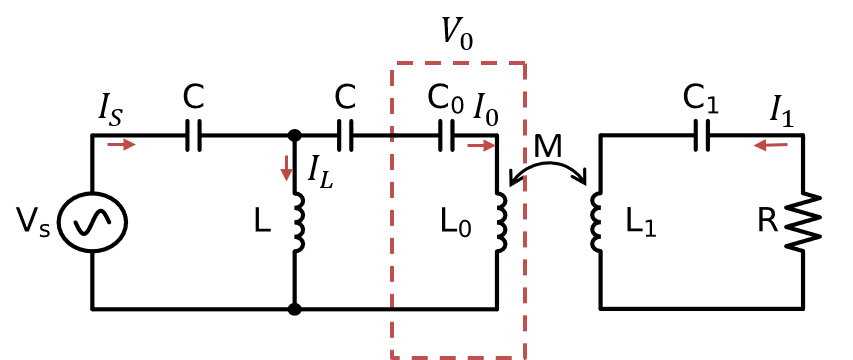
\includegraphics[width=0.8\linewidth]{images/3_clc_s_scheme.png}
%     \caption{CLC-S Scheme.}
%     \label{fig:3_clc_s_scheme}
% \end{figure}